% !TEX root = ../../main.tex

\section{Materials and methods}

\subsection{Materials}

The UiO-66(Zr) \gls{MOF} used in this study was synthesised according
to the procedure described in \autoref{appx:synthesis:uio66def},
which was adapted from \citet{shearerTunedPerfectionIroning2014}.
This particular method was chosen to ensure that a structure with
a minimal number of intrinsic defects would be obtained.

The resulting parent \gls{MOF} was activated for \SI{8}{\hour} at
\SI{200}{\degreeCelsius} to ensure that all solvent was removed.
\SI{200}{\milli\gram} aliquots of material were prepared and 
placed in vials, alongside the monotopic acid dissolved in
\SI{20}{\milli\litre} of the respective solvent. The quantities
of acid correspond to molar quantities of the framework.
The samples were then gestated over a \SI{24}{\hour} period
at \SI{80}{\degreeCelsius} in a temperature controlled oven.
Pressure resistant Schott sealed bottles were used to ensure that
solvents with a lower boiling point do not evaporate.
After leaching, samples were collected and washed in ethanol
for \SI{4}{\hour}, a procedure repeated 4 times. Finally, all 
samples were dried at \SI{120}{\degreeCelsius}.

\begin{figure}[htb]
	\centering
	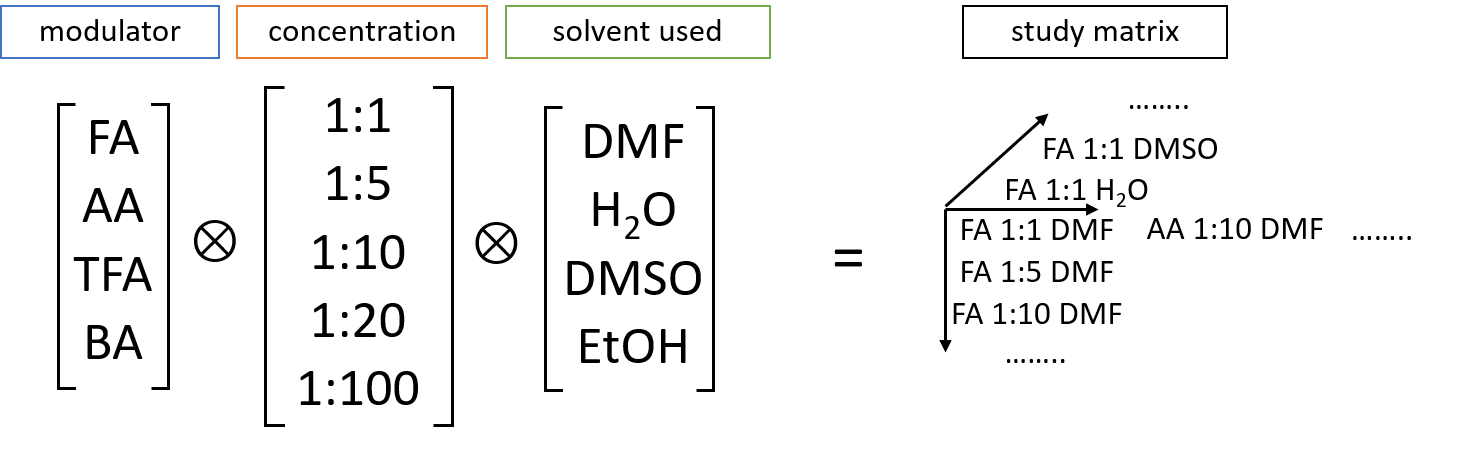
\includegraphics[width=\linewidth]{study-matrix}%
	\caption{The matrix of this study.
	}\label{def:fig:study-matrix}

\end{figure}

To generate a comprehensive map of the influence
of different variables on defect concentration, a number of
leaching conditions have been selected. The same monotopic acids 
which have been successfully used
as modulators in the synthesis of defective UiO-66
(\gls{FA}, \gls{AA}, \gls{TFA} and \gls{BA}) 
were used in various concentration ranges,
from 1 to 100 molar equivalents with respect to the framework.
In order to verify the contribution of the solvent,
\gls{DMF}, deionized water, ethanol and \gls{DMSO} 
were used as the leaching medium, generating a matrix of 
studied factors as seen in \autoref{def:fig:study-matrix}
Two parent materials have been synthesised, PWI-C which formed 
the basis of the initial \gls{DMF} test trial, and JM237 which 
was made in bulk to be used for subsequent solvent batches.
The \gls{DMF} dataset does not include any trifluoroacetic acid
leached samples, as it was only used in the latter sample sets.
Furthermore, no benzoic acid samples could be generated when using
water as a solvent, due to its poor solubility. Finally, 
at high acid concentrations, several of the samples were completely
dissolved during leaching
conditions. The mass loss during leaching was found to be 
between 10 and 60\%, depending on the acid and solvent used.
When using 10 equivalents of \gls{TFA} in \gls{DMSO}, only 18\% of the 
original sample could be recovered. 
A summary of all generated materials can be found in
\autoref{def:tbl:samples}.
Some properties of the acids and solvents used, such as acidity,
solubility, etc.\ are found in 
\autoref{appx:def:tbl:acid} and \autoref{appx:def:tbl:solvent} of 
\autoref{appx:def} respectively.

\begin{table}[p]
	\centering\footnotesize
	\caption{Samples used in the UiO-66(Zr) linker leaching study}
	\begin{tabular}{lcccc}
		\toprule
		\textbf{Sample name}
		      & \textbf{Solvent}
		      & \textbf{Modulator}
		      & \textbf{Concentration}
		      & \textbf{Observations}                                            \\
		\midrule
		PWI-C & None                   & None     & None  & Parent material      \\
		FA1   & DMF                    & \gls{FA}  & 1:1   & ---                  \\
		FA5   & DMF                    & \gls{FA}  & 1:5   & ---                  \\
		FA10  & DMF                    & \gls{FA}  & 1:10  & ---                  \\
		FA20  & DMF                    & \gls{FA}  & 1:20  & ---                  \\
		FA100 & DMF                    & \gls{FA}  & 1:100 & ---                  \\
		AA1   & DMF                    & \gls{AA}  & 1:1   & ---                  \\
		AA5   & DMF                    & \gls{AA}  & 1:5   & ---                  \\
		AA10  & DMF                    & \gls{AA}  & 1:10  & ---                  \\
		AA20  & DMF                    & \gls{AA}  & 1:20  & ---                  \\
		AA100 & DMF                    & \gls{AA}  & 1:100 & ---                  \\
		BA1   & DMF                    & \gls{BA}  & 1:1   & ---                  \\
		BA5   & DMF                    & \gls{BA}  & 1:5   & ---                  \\
		BA10  & DMF                    & \gls{BA}  & 1:10  & ---                  \\
		BA20  & DMF                    & \gls{BA}  & 1:20  & ---                  \\
		BA100 & DMF                    & \gls{BA}  & 1:100 & Completely dissolved \\
		JM237 & None                   & None      & None  & Parent material      \\
		JM328 & \ce{H2O}               & \gls{FA}  & 1:10  & ---                  \\
		JM329 & \ce{H2O}               & \gls{FA}  & 1:100 & ---                  \\
		JM330 & \ce{H2O}               & \gls{AA}  & 1:10  & ---                  \\
		JM331 & \ce{H2O}               & \gls{AA}  & 1:100 & ---                  \\
		JM332 & \ce{H2O}               & \gls{BA}  & 1:10  & ---                  \\
		JM333 & \ce{H2O}               & \gls{BA}  & 1:100 & ---                  \\
		JM334 & \ce{H2O}               & \gls{TFA} & 1:10  & ---                  \\
		JM335 & \ce{H2O}               & \gls{TFA} & 1:100 & ---                  \\
		JM351 & MeOH                   & \gls{FA}  & 1:10  & ---                  \\
		JM352 & MeOH                   & \gls{FA}  & 1:100 & ---                  \\
		JM353 & MeOH                   & \gls{AA}  & 1:10  & ---                  \\
		JM354 & MeOH                   & \gls{AA}  & 1:100 & ---                  \\
		JM355 & MeOH                   & \gls{BA}  & 1:10  & ---                  \\
		JM356 & MeOH                   & \gls{BA}  & 1:100 & ---                  \\
		JM357 & MeOH                   & \gls{TFA} & 1:10  & ---                  \\
		JM358 & MeOH                   & \gls{TFA} & 1:100 & ---                  \\
		JM359 & MeOH                   & None      & 0     & Control              \\
		JM360 & DMSO                   & \gls{FA}  & 1:10  & ---                  \\
		JM361 & DMSO                   & \gls{FA}  & 1:100 & ---                  \\
		JM362 & DMSO                   & \gls{AA}  & 1:10  & ---                  \\
		JM363 & DMSO                   & \gls{AA}  & 1:100 & ---                  \\
		JM364 & DMSO                   & \gls{BA}  & 1:10  & ---                  \\
		JM365 & DMSO                   & \gls{BA}  & 1:100 & ---                  \\
		JM366 & DMSO                   & \gls{TFA} & 1:10  & ---                  \\
		JM367 & DMSO                   & \gls{TFA} & 1:100 & Completely dissolved \\
		JM368 & DMSO                   & None     & 0     & Control              \\
		\bottomrule
	\end{tabular}%
	\label{def:tbl:samples}
\end{table}%

\subsection{Methods for quantifying defects}

Determining the abundance of missing linker and missing cluster 
defects and characterising their distribution is a major challenge,
as the components of the framework to not change, only their local
order.

If the distribution of defects can introduce changes in the
long-range order and topology of the parent framework,
such as by the introduction of phase changes,
additional peaks can be observed through regular
powder diffraction techniques.
As~\citet{cliffeCorrelatedDefectNanoregions2014} has shown,
the UiO-66 defect-free face-centred unit (\textbf{fcu})
net can be transformed through missing cluster defects into
a (\textbf{reo}) net. Short-range correlations of such domains
form nanoregions inside the parent structure and generate
diffuse scattering peaks observable at low angles in
\gls{pXRD}, corresponding to ``forbidden''
reflections in a primitive cubic superstructure.
As such, these \gls{pXRD} peaks can be used to verify the existence of
missing cluster defects, but only when their abundance allows for
nanodomains of (\textbf{reo}) nets to be formed. In this study,
\gls{pXRD} measurements were performed as described in \autoref{appx:char:pxrd}
as quick screening for a large degree of defectivity.

One of the most accessible ways of assessing the defectivity of
a \gls{MOF} is thermogravimetry (\gls{TGA}). Through heating in
an oxygen-rich atmosphere, the \gls{MOF} is normally reduced to
its metal oxide, and a stoichiometric analysis of the \gls{TGA} curve
can allow for the percentage of missing linkers per cluster to be
determined. \gls{TGA} curves for this study were measured under
an air atmosphere using the method described in \autoref{appx:char:TGA}.
A heating rate of \SI{5}{\degreeCelsius\per\minute} was used.
The curves are then normalized with respect to the weight at
\SI{600}{\degreeCelsius}, which corresponds to pure
\ce{ZrO2}. The maximum possible mass loss of a solvent-free
structure is calculated from the ratio of the fully-substituted,
but dehydroxilated, metallic cluster \ce{Zr6O6(C6H4(COO)2)6}. The plateau
of the \gls{TGA} curve between \SIrange{400}{500}{\degreeCelsius},
in the range where it is assumed that the molecules included in
the framework are completely evacuated, is used as a measure of the
number of terephtalate linkers which are missing.

In order to check for the inclusion of a modulator in the framework,
the \gls{MOF} can be digested with the help of a hydrofluoric acid and the
resulting solution can be analysed through proton (\ce{^{1}H}) \gls{NMR} 
or \gls{HPLC}. Unfortunately, due
to constraints in equipment availability,
the results of these studies are not yet available for these samples.

Finally, both nitrogen adsorption at \SI{77}{\kelvin} and \ce{CO2}
adsorption at \SI{303}{\kelvin} can be used to describe the surface
characteristics and porosity of the samples. The methods for obtaining
the isotherms are presented in detail in \autoref{appx:char:N2phys}
and \autoref{appx:char:highthroughput} for \ce{N2} and \ce{CO2}
respectively.